\documentclass[a4paper]{article}

\usepackage[english]{babel}
\usepackage[utf8x]{inputenc}
\usepackage{amsmath}
\usepackage{graphicx}
\usepackage[colorinlistoftodos]{todonotes}
\newcommand{\pder}[2]{\frac{\partial#1}{\partial#2}}
\setlength\parindent{0pt}

\title{CSE250B Project 1}
\author{Mehmet Koc A53035914\\Zeynep Su Kurultay A53034989}

\begin{document}
\maketitle


\begin{abstract}
In this project, we train a regularized logistic regression classifier with two optimization methods, namely stochastic gradient ascent (SGA) and L-BFGS. The best regularization strength is chosen via grid search on a validation set, independent from the actual training set. Then, the trained model is tested with the best regularization parameter on a separate test set. Both training and test sets are obtained from Gender Recognition [DCT] dataset from MLComp \cite{Label1}. The results for the two methods are presented and plotted against epochs and/or grid-searched values, respectively.
\end{abstract}

\section{Introduction and Theory}

 The logistic regression model has the following formula:
 \\$$p = P(y=1|x;\beta) = \sigma(\beta^{T}X) = \frac{1}{1+e^{-\beta^{T}X}}$$\\
 where $\beta_0$ is intercept and $x_0 = 1$ is pseudo-feature.
 Two important properties of logistic regression are:\\\\
 1) $P(y=-1|x;\beta)=1-p=\sigma(-\beta^{T}x)$\\
 2) $\pder{(\sigma (z))}{z} = \sigma(z) \sigma(-z)$\\
 
 Having a training set $D = \{x_i , y_i\}_{i=1}^{n}$ and assuming $y_i$'s are conditionally independent given $x_i$, the objective is to find $\beta^*$ that maximizes log-conditional-likelihood (LCL) with regularization (RLCL):
 $$\beta^{*} = \max_{\beta} - \sum_{i=1}^{n} log(1+e^{-\beta^{T}x_{i}y_{i}}) - \mu \beta^{T} \beta = \max_{\beta} LCL - \mu ||\beta||_{2}^{2} = \max_{\beta} RLCL $$
 
 The objective above tries to find the optimal $\beta$ for training data while keeping $||\beta||_{2}$ bounded. Here, Euclidean norm is selected due to its mathematical convenience. $\mu$ is the parameter that sets the strength of regularization and best $\mu$ can be found by sparing a validation set in the training data (i.e. validation). \\\\
 
 Due to the nonlinearity of logistic function, it is hard to obtain the closed-form solution by solving $\pder{(RLCL)}{\beta} = 0$. Due to this fact, two numerical optimization techniques are employed, and their details are discussed below.
 
\subsection{Stochastic Gradient Ascent}
 
Gradient ascent (GA) is one method that is used to find the extremum in the logistic function, where $\lambda$ is the learning parameter (step size):
 
 $$\beta_{k+1} \longleftarrow \beta_k + \lambda \pder{(RLCL)}{\beta} \bigg|_{\beta=\beta_k} \Longleftrightarrow \beta_{k+1} \longleftarrow \beta_k + \lambda (\sum_{i=1}^{n} (y_i - p_i) x_i - \mu \beta_k) $$
 
Note that the factor 2 coming from the derivative is merged into $\mu$ and this should be kept in mind while interpreting $\mu$ values. The time complexity of one update of the rule above is O(nd) (assuming that the computation of logistic function is O(1)) in the general case where d is the dimension of the feature space and n is the number of training examples. The space complexity is linear (i.e. O(d)) since $\beta_k$ requires O(d) space and x and y are already allocated inputs. This space complexity assumes $p_i$ is not stored. \\
 
To make GA faster, stochastic gradient ascent (SGA) can be used  where training data is sorted randomly and one example at a time is used in the following stochastic update rule for 3-100 epochs \cite{Label2} or until convergence.
 
 $$\beta_{k+1} \longleftarrow \beta_k + \lambda ((y_i - p_i) x_i - \mu \beta_k)$$

Time complexity of one stochastic update is O(d) (compared to O(nd) of standard GA) and the space complexity remains the same compared to standard GA. In addition, for learning rate and regularization to treat each feature similarly, it is desirable to normalize the features by z-scoring. Note that z-scoring is more robust to noisy values compared to [0, 1] normalization.

$$ x_i \longleftarrow \frac{x_i - \mu_i}{\sigma_i}\, for\, i=1,2,...,d$$

Note that the affine mapping above makes each feature of mean ($\mu_i$) 0 and variance ($\sigma_i^2$) 1. It is important to use the same $\mu_i$ and $\sigma_i$ while normalizing the test set. 
\\\\
Best $\mu$ can be selected by creating a validation set in the training data independent of the actual training set (i.e. the part of training data used for training). The objective here is to choose $\mu$ that maximizes LCL on the validation set $\{x_i , y_i \}_{i=1}^{t}$ where $t < n$.
$$LCL_{validation} = \sum_{i=1}^{t}log(p_i)\; where\; p_i = \frac{1}{1+e^{-\beta^{T}x_i y_i}}$$

The formulation above causes overflow/underflow problems. For example, when $\beta^{T}x_i y_i$ becomes very small $p_i \rightarrow 0;\, logp_i \rightarrow -\infty$ and this prevents us from selecting best $\mu$. The solution for this is:

\begin{equation*}
LCL_{validation} = \sum_{i=1}^{t}l_i\; where\; l_i 
\begin{cases}
-log(1+e^{-\beta^T x_i y_i}), & \text{if}\ \beta^T x_i y_i \ge 0 \\
\beta^T x_i y_i - log(1+e^{\beta^T x_i y_i}), & \text{otherwise}
\end{cases}
\end{equation*}

\subsection{L-BFGS}

We also use minFunc \cite{Label3}, as mentioned in the project description, in order to obtain an optimization on the logistic function. Since we do not have to delve too deeply into the mathematical details, we will mention the general idea and usage of this algorithm. L-BFGS, which is the method to be used by minFunc when searching the minimum value of the input function, achieves optimization of this input function using line-search methods. The original function, BFGS implements Newton's method in optimization, which is an iterative method whose greatest difference to gradient descent is that it uses curvature information of the input function to achieve a more direct and monotonic route \cite{Label6}. The difference between BFGS and L-BFGS (which actually stands for Limited memory BFGS) is that it stores the approximation in an implicit manner with much fewer information than BFGS, but in an equally representative manner. This is important since implementing BFGS requires taking the computing and taking the inverse of Hessian matrix which is $O(n^3)$ and is very time-costly. \\

It is possible to talk about the time and space complexity of minFunc on a fairly high level. It has a parameter called progTol, which stands for progress tolerance, and this parameter serves as a termination condition for the program. If the input function to minFunc is a function that decreases very slowly, minFunc would theoretically iterate more times. The space complexity is less complicated, and L-BFGS, as mentioned, is an optimization over the actual function, BFGS, over space. L-BFGS, unlike BFGS, stores the approximation in linear storage.

\section{Experiments}

For the purposes of this project, we use the Gender Recognition [DCT] dataset from MLComp \cite{Label1}. The dataset has 559 training and 239 test examples. The dataset has 800 columns the first of which is the label (i.e. 1 for positives or -1 for negatives) for tuples and the remaining 799 are predictors. Pseudo-vector $x_0 = 1$ is added to these 799 predictors and overall number of predictors becomes 800. The base rate in the training set is 0.49 whereas the base rate in the test set is 0.51. First, we analyze the features of the dataset at hand in order to get a better view of what we are handling. We extract the minimum, maximum, mean and standard deviation (sd) statistics of the training data (The measures in the test set are similar). Furthermore, we examine the sparsity and number of unique values in training data (Sparsity defined in [0, 1] range where 1 means all feature values being non-zero). These statistics are summarized in Fig.~\ref{fig:stats}.\\

From Fig.~\ref{fig:stats}, it is observed that about the first 320 features are small in value (another point showing the importance of normalization) and they are highly sparse. Moreover, these features generally have quite few distinct values (e.g. some of them only have 4 distinct values) by Fig.~\ref{fig:stats}(f). This observation suggests that such features are likely to be categorical features and hence, they need recoding. However, since we do not have any information on the meaning of features, we do not apply any recoding on data and we apply only normalization. Normalization on the original numerical data is done by z-scoring so that the resultant distribution is with mean 0 and sd 1, as explained in the theory section. \\

\begin{figure}
  \makebox[\textwidth][c]{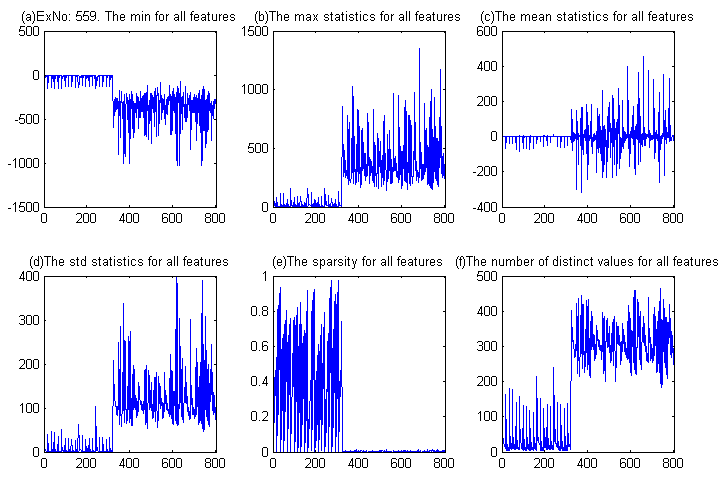
\includegraphics[width=1.2\textwidth]{1_featStats.png}}%
  \caption{Statistics of the training set of the dataset}
  \label{fig:stats}
\end{figure}

Maximizing RLCL requires finding a good value for $\mu$. For this purpose, we split the training set of the original dataset into validation set and actual training set. We use 30\% randomly chosen portion of the original training set as the validation set. According to that, there are 392 actual training examples and 167 validation set examples. A number of values for $\mu$ growing exponentially are chosen and the best $\mu$ is picked via grid search, as explained in \cite{Label4}. The values for $\mu$ we used is for SGA; 2.\^{}{[}-1.0:0.2:1.4{]} and for L-BFGS; 2.\^{}{[}-1.0:0.5:2.0{]}.

\subsection{SGA Details}

For SGA, as reasoned in the Theory section, we use 7 epochs (EpochNum = 7) without early stopping; since dataset is small and hence SGA takes a short time. Also, a small constant learning rate $\lambda_0 = 0.1$ that exponentially decays with each epoch is used (since the improvement with each new epoch is smaller):

$$ \lambda = \lambda_0 * 0.9^{j-1} \; where \; j = 1, 2,..., EpochNum$$

In each epoch, the training examples are randomly sorted. At each update of SGA, one example is used and $\beta$ and $p_i$ are updated. After all training examples are used, the implementation is continued with the next epoch. The starting point for $\beta$ is 0 vector.

\subsection{L-BFGS Details}

A similar approach is taken when implementing L-BFGS. The L-BFGS function obtained from \cite{Label3} is supplied with our RLCL function and the gradient function of RLCL is also computed, as explained in the Theory section, and passed in as an argument. Different options that minFunc presents are examined, and we decide to change some of the options. The method is set to 'lbfgs' while the option that disables mex usage is set to 1. This is done since the function is already fast, there is no need to use the pre-compiled mex files. The numDiff option is not changed, since we supply our own gradient function. We also see no need to change the step length and the progress tolerance, since the accuracy we obtain at the end is quite high.\\

Different from SGA, checkgrad2.m \cite{Label5} is used in order to verify that the gradient function that is supplied to minFunc is correct. Checkgrad2 is a function that uses a single direction to check the gradient vs. change in objective. The output of checkgrad2.m should ideally be close to unity, since the ratio of change of objective to directional gradient is expected to be 1. We obtain 1.0 as an output, and hence conclude that our gradient function is correct. The training portion of the data is used in order to obtain the optimum $\mu$. The best $\mu$ value is selected according to the maximum RLCL value and is used on the validation set. The LCL and accuracy is measured on the validation set and best $\mu$ is picked up similar to what is done for SGA.

\section{Results}

\subsection{SGA Results}

We present the variation of LCL for validation set in Fig.~\ref{fig:lclvsep}, in three graphs. In each graph, the x axis is the epoch number and each LCL variation curve corresponds to one $\mu$ value in grid search. The first graph shows log(-LCL) vs epoch number in log scale. Since $LCL < 0$ and we want to maximize LCL, the lowest log(-LCL) value is favorable. Hence we get rid of the last two $\mu$ values that result in very poor LCL and plot the rest of Fig~\ref{fig:lclvsep}(a) in Fig~\ref{fig:lclvsep}(b). The very poor results for the last two $\mu$ values indicates the dependence of convergence of SGA on the learning rate. The third graph is not plotted on log scale unlike the first two graphs, and it shows the negative of the actual LCL values and it is seen that LCL values generally converge after the third epoch. So, it is concluded that using $epochNum = 7$ is more than enough. These three graphs display the convergence of LCL values as SGA iterates. By Fig~\ref{fig:lclvsep}(c), the best LCL is obtained at $\mu = 2$.\\

\begin{figure}
\makebox[\textwidth][c]
{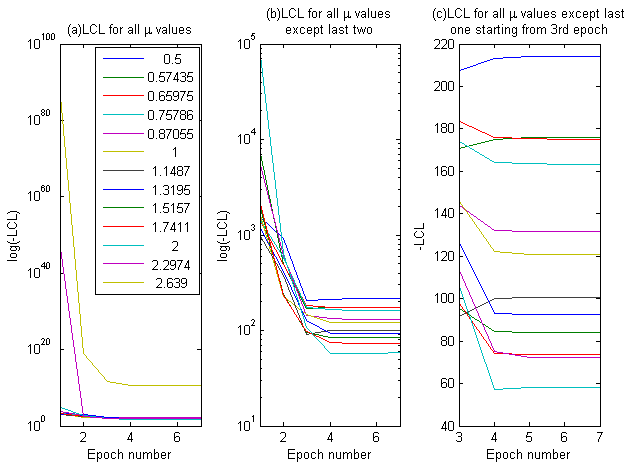
\includegraphics[width=1.2\textwidth]{2_LCLvsEpochNum.png}}
\caption{\label{fig:lclvsep}LCL vs Epoch numbers for SGA implementation}
\end{figure}

0/1 accuracy is a good metric to evaluate performance for this dataset since the number of examples from each class are balanced. The 0/1 accuracies obtained on the validation set can be seen in Fig.~\ref{fig:valacc}. The accuracy is plotted against the epoch numbers. The first graph shows all of the values the 0/1 accuracy takes, and the second graph is a close-up version that depicts the convergence point for accuracy values. By Fig.~\ref{fig:valacc}(b), the best accuracy is obtained at $\mu = {1.15, 1.52}$ with 86.8\% accuracy. This shows that the $\mu$ value that maximizes LCL ($\mu = 2$) on the validation set is not necessarily the same $\mu$ value that maximizes 0/1 accuracy. The accuracy of $\mu = 2$ being 86.2\% accuracy is still very close to the maximum accuracy obtained. In the end, $\mu = 2$ is chosen since the starting objective was to maximize regularized LCL. The resulting accuracy statistics can be seen in Table ~\ref{tab:sgatable}, where true positives, false positives, true negatives and false negatives are displayed with their initials and corresponding values, respectively.\\

\begin{figure}
\makebox[\textwidth][c]
{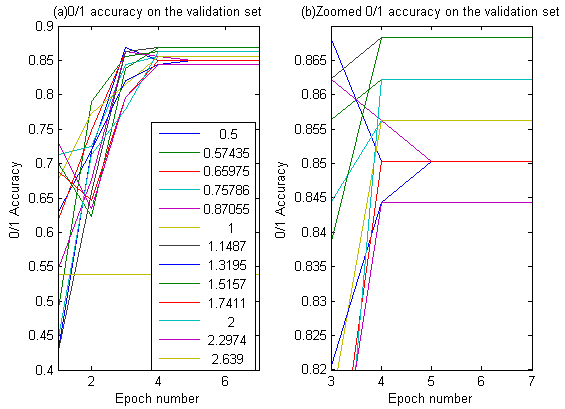
\includegraphics[width=1.2\textwidth]{3_validationAcc.png}}
\caption{\label{fig:valacc}0/1 accuracies on the validation set vs Epoch Number for SGA}
\end{figure}



\begin{table}
\centering
\begin{tabular}{l|r}
Type & Count \\\hline
tp & 111 \\
fp & 14 \\
tn & 102 \\
fn & 12
\end{tabular}
\caption{\label{tab:sgatable}Accuracy statistics on the test set for SGA.}
\end{table}

The 0/1 accuracy in the test is observed to be 89.1\%. Note that this is a bit unusual since the maximum 0/1 accuracy obtained on the validation set was 86.8\%. Although normally one expects worse performance on the test set than the validation set, the discrepancy can be attributed to the small validation (167 examples) and test sets (239 examples) and the fact that validation was applied instead of cross-validation. 

\subsection{L-BFGS Results}

We construct graphs similar to those of SGA (by Fig.~\ref{fig:lclvsep}-~\ref{fig:valacc}) part for the L-BFGS part, as can be seen in Fig.~\ref{fig:lbfgsglcl}. LCL values are similarly plotted in a log scale for the first graph and the negative of the actual values are plotted in the second graph. Note that the LCL values are plotted against the $\mu$ values this time (no epochs). Also note that from Fig.~\ref{fig:lbfgsglcl} that the best LCL is obtained at $\mu = 8$. This trend of LCL in Fig.~\ref{fig:lbfgsglcl} before $\mu \leq 2$ is similar to that in Fig.~\ref{fig:lclvsep}. There is a significant difference after $\mu > 2$ and this can be attributed to constant learning rate of SGA. This shows the superiority of L-BFGS over SGA since it utilizes the curvature of the objective function. Note that we could have also included $\lambda$ in the grid-search, but we did not intentionally since it better shows the superiority of L-BFGS over SGA. Doing so would also make the grid-search 2D (searching for both $\mu$ and $\lambda$), hence taking more time.\\

\begin{figure}
\makebox[\textwidth][c]
{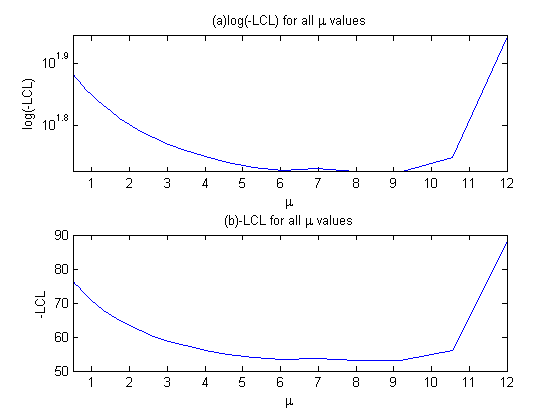
\includegraphics[width=1.2\textwidth]{4_LCLvsMu.png}}
\caption{\label{fig:lbfgsglcl}LCL vs $\mu$ for L-BFGS implementation}
\end{figure}

The accuracies obtained from different $\mu$ values by Fig.~\ref{fig:lbfgsglcl} are very close to each other. This is expected since the LCL vs $\mu$ values are also very close to each other. Similar to what is done for SGA, we again measure the 0/1 accuracy this time for L-BFGS. In the validation set, the best accuracy is observed to be 89.2\% while in the test set it is observed to be 90.2\%. The resulting accuracy statistics for L-BFGS can be seen in Table ~\ref{tab:lbfgstable}, where true positives, false positives, true negatives and false negatives are displayed with their initials and corresponding values, respectively.\\

\begin{table}
\centering
\begin{tabular}{l|r}
Type & Count \\\hline
tp & 109 \\
fp & 13 \\
tn & 103 \\
fn & 14
\end{tabular}
\caption{\label{tab:lbfgstable}Accuracy statistics on the test set for L-BFGS.}
\end{table}

In Table  ~\ref{tab:timet}, the mean time of each of the two algorithms over 20 iterations is depicted. As can be seen, on average, L-BFGS takes about twice the time as SGA. 

\begin{table}
\centering
\begin{tabular}{l|r}
SGA & L-BFGS \\\hline
0.11160 & 0.216326
\end{tabular}
\caption{\label{tab:timet}Mean execution time of two approaches}
\end{table}

\section{Conclusion}

In conclusion, we first perform the necessary transformations on data (i.e. normalization) and split the data into separate actual training and validation sets. Then, in order to ensure that RLCL is maximized in the best way possible; we use grid search to find the best $\mu$ on the training set to be used on the validation set. For SGA, we use 7 epochs and a decaying learning rate and obtain the highest values of LCL and measure the accuracy. For L-BFGS, we test different $\mu$ values and find the optimal value. It is interesting to note that the performance on the validation set for $\mu$ close to 0 (i.e. no regularization) is reasonable for both methods although it is not the best. The accuracies obtained on the test set are 89.1\% and 90.2\% for SGA and L-BFGS, respectively. L-BFGS achieves a slightly higher accuracy due to the fact that it does not require an optimum selection for learning rate. The accuracy of SGA could be increased if an additional grid-search over the learning rate is performed, but since the accuracy is very close to that of L-BFGS and since doing grid-search in more than one dimension would increase the complexity; we decide not to implement this approach. This way, it is also better to indicate the more superior qualities of L-BFGS over SGA.\\

In order to improve the accuracies, fine-tuning the learning rate of SGA is required, as explained; but even with an optimal learning rate, these algorithms might not be able to reach the given highest accuracy on the MLComp website \cite{Label1}, which is an error rate of 0.084 achieved by svmlight-linear. This can be attributed to the fact that hinge loss (the loss function for SVM) is better way to express cost for this dataset. The better accuracy could have been reached though if we knew the meanings of features and recoded them accordingly.\\

In a nutshell, the optimal $\mu$ values found using both SGA and L-BFGS approaches are very close, as expected; and both achieve fairly high accuracy on the given dataset. These results are consistent, as can be seen by Table~\ref{tab:sgatable} and Table~\ref{tab:lbfgstable} and in line with our expectations.

\begin{thebibliography}{99}
\bibitem{Label1} http://archive.ics.uci.edu/ml/datasets/Adult.
\bibitem{Label2} http://cseweb.ucsd.edu/~elkan/250B/logreg.pdf.
\bibitem{Label3} http://www.di.ens.fr/~mschmidt/Software/minFunc.html
\bibitem{Label4} C. C. Chang and C. J. Lin.LIBSVM: a library for support vector machines. ACM Transactions on Intelligent Systems and Technology, 2:27:127:27, 2011. Software available at http://www.csie.ntu.edu.tw/ cjlin/libsvm. Theory, pages 144152. ACM Press, 1992.
\bibitem{Label5} http://people.csail.mit.edu/jrennie/matlab/checkgrad2.m
\bibitem{Label6} http://www.nd.com/NSBook/NEURAL20AND20ADAPTIVE20SYSTEMS18\_Newtons\_Method.html
\end{thebibliography}

\end{document}